Der Begriff CRUD steht für Create, Read, Update und Delete. Dies sind vier grundlegende Operationen in der Datenverarbeitung. Oft bilden diese Operationen die grundlegende Schnittstelle zwischen Andwendungen und Datenbanken.
\newline
\begin{figure}[h!]
    \centering
    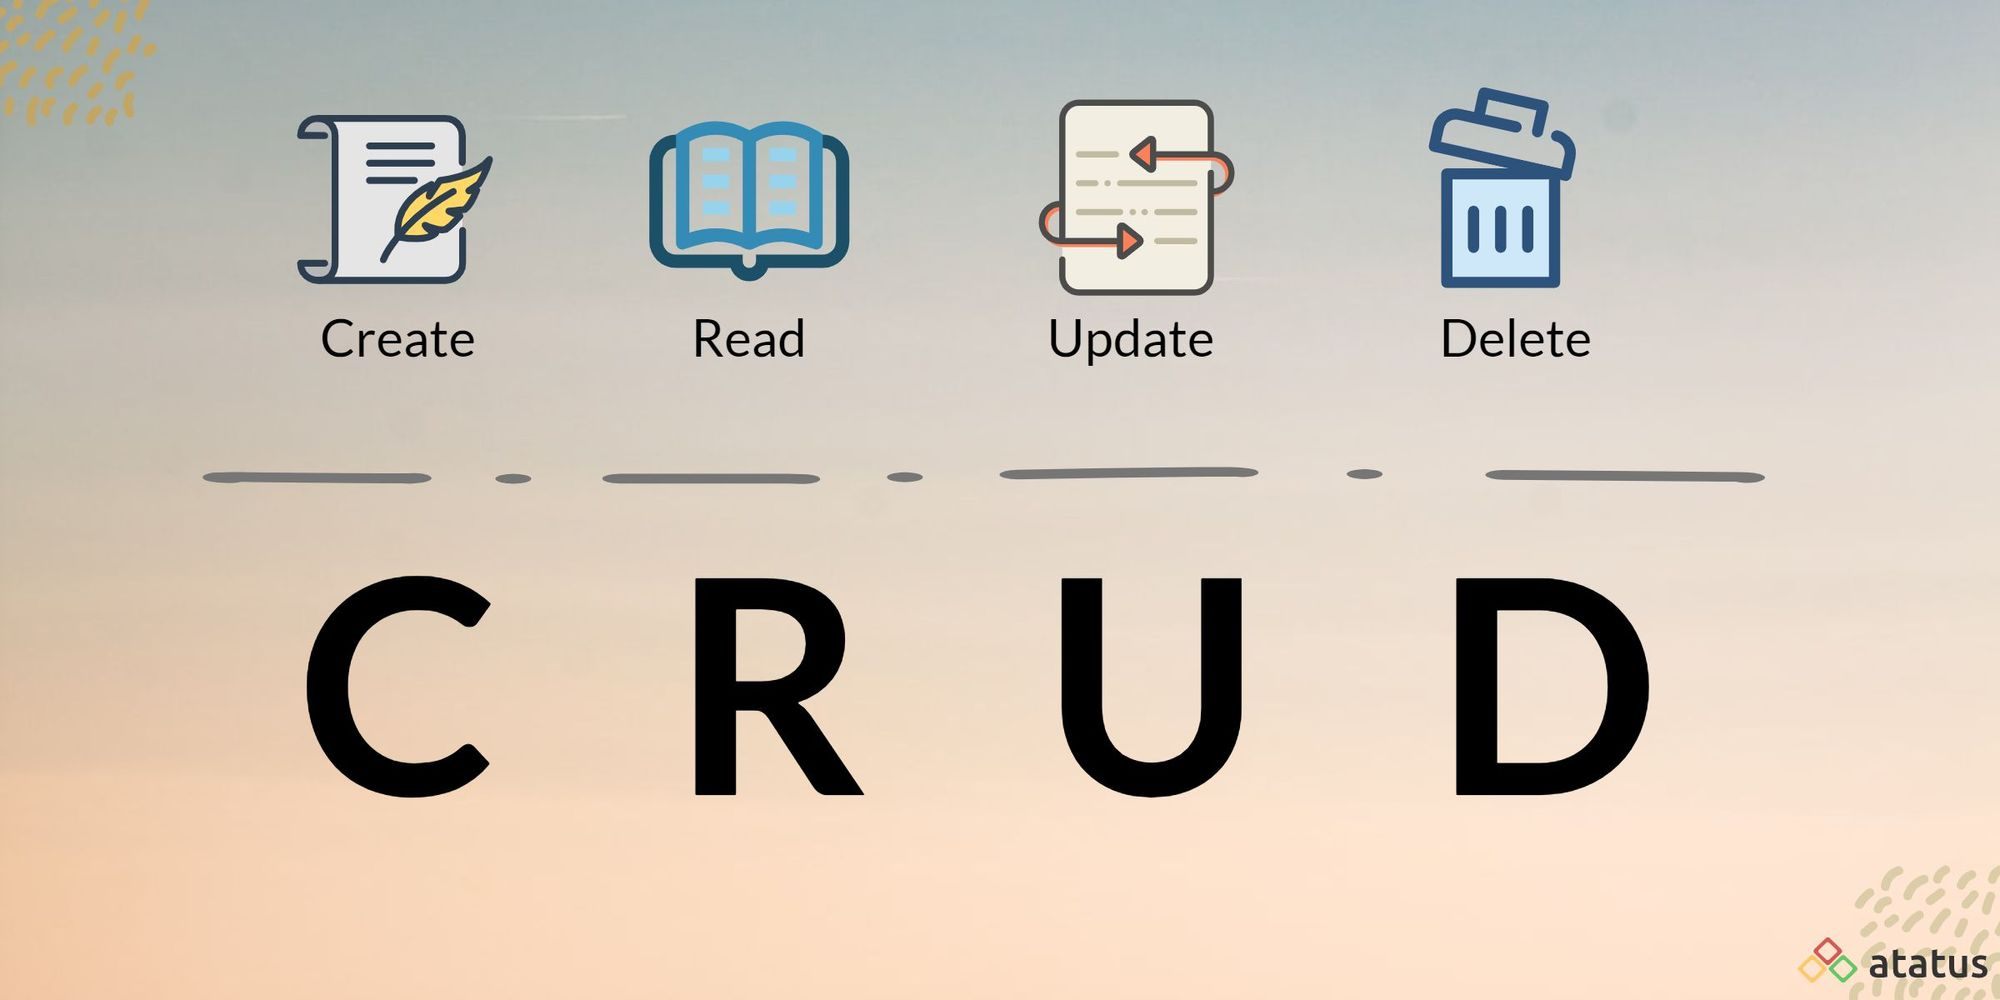
\includegraphics[width=0.8\textwidth]{pics/CRUD.jpeg}
    \caption{CRUD Operations}
    \label{fig:enter-label}
\end{figure}


 \subsection{Create}

 Bei der Create Operation geht es darum, neue Daten in die Datenbank zu persistieren. Es können beispielsweise neue Benutzer:innen oder Pläne angelegt werden.


 \subsection{Read}

 Die Read-Operation ergmöglicht es, vorhandene Daten aus der Datenbank auszulesen. Dies erfolgt in der Form von Abfragen, um Datensätze nach bestimmten Kritierien zu filtern, oder gegebenenfalls auch alle Datensätze abzurufen.

\begin{lstlisting}[caption=Read-Operation]
async function getProjectById (id) {
  if (!id) {
    throw new Error('ID must be provided')
  }
  const collection = planfredDbReadOnly.db.collection('projects')

  try {
    return collection.findOne({ _id: new ObjectId(id) })
  } catch (err) {
    throw new Error(err)
  }
}
\end{lstlisting}

Dieses Code Beispiel ist eine asynchrone Funktion names "getProjectById" welche ein Projekt anhand der ID aus der Datenbank ausliest.\newline
Zu Beginn wird überprüft, ob eine ID übergeben wurde. Falls nicht, wird mittels des "Early Return Pattern" sofort ein Fehler ausgelöst. Wenn die ID korrekt übergeben wurde, wird die entsprechende Collection, in diesem Fall "projects", in einer Variable gespeichert. Anschließend wird versucht, das entsprechende Projekt mit Hilfe eines Try-Catch-Statements abzurufen. Auch hier gilt wieder, sollte irgendwo in diesem Code Block ein Fehler vorkommen wird sofort ein Fehler ausgelöst.



\subsection{Update}

Die Update-Operation wird verwendet, um bereits bestehende Datensätze in der Datenbank zu verändern. Das können beispielsweise Anpassungen von Adressen in einer Kundendatenbank, oder Preisänderungen in einer Produktdatenbank sein. Ähnlich wie bei READ-Operationen können UPDATE-Operationen, abhängig von den ausgewählten Kriterien, auf sämtliche Datensätze, oder nur auf ausgewählte beschränkt werden.

Manche Big-Data-Systeme verzichten gänzlich auf die Integration der UPDATE-Operation und ermöglichen stattdessen ausschließlich eine CREATE-Operation in Verbindung mit einem Zeitstempel. Dabei wird bei jeder Aktualisierung eine neue Version der Zeile hinzugefügt.

\begin{lstlisting}[caption=Update-Operation]
try {
    const response = await fetch(`${config.planfredApiUrl}crm/projects/` + req.params.id, {
      method: 'PATCH',
      headers: {
        'Content-Type': 'application/json'
      },
      body: JSON.stringify(req.body)
    })
    const responseJSON = await response.json()
    return res.json(responseJSON)
  } catch (e) {
    console.error(e)
  }
\end{lstlisting}
\newpage
Dieses Code Beispiel verwendet die Node.js Fetch API. 

\begin{lstlisting}
    const response = await fetch(`${config.planfredApiUrl}crm/projects/` + req.params.id, {method: 'PATCH' })
\end{lstlisting}

In diesem Teil wird ein API-Aufruf mit fetch() durchgeführt, um die angegebene Ressource zu aktualisieren. Die URL für den API-Aufruf wird durch Verketten von config.planfredApiUrl, dem Teil der URL für die API, und req.params.id, dem Parameter aus der Anfrage, erstellt. Der API-Aufruf wird mit der Methode 'PATCH' ausgeführt, um eine partielle Aktualisierung der Ressource durchzuführen. Die Anfrage erfolgt asynchron, da "await" verwendet wird, um auf die Antwort zu warten.\newline

Im nächsten Teil werden die Headers gesetzt. In diesem Fall wird der "Content-Type" Header auf "application/json" gesetzt. Somit kann als Rückgabe Wert ein JSON Objekt zurückgegeben werden. Im Body wird der Inhalt der Anfrage festgehalten, hier wird JSON.stringify verwendet, um die Daten in ein JSON Format zu konvertieren, welches von der API erwartet wird.

\subsection{Delete}


Die DELETE-Operation erlaubt es den Nutzer:innen, Datensätze aus der Datenbank zu löschen. Bei einem endgültigen Löschen wird der Datensatz vollständig entfernt, während er beim vorläufigen Löschen markiert wird, aber an seinem aktuellen Ort bleibt.



In dieser Diplomarbeit wurden hauptsäclich READ und UPDATE-Operations verwendet. Die Syntax um ein Projekt zu löschen sieht wie folgt aus.

\begin{lstlisting}[caption=Delete-Operation]
    const project = await Projects.findById(req.params.id)

  try {
    project.trashed = req.body.value.new
    project.trashedDate = new Date()

    await project.save()

    res.json({ success: true })
  } catch (e) {
    next(e)
  }
\end{lstlisting}

Zu Beginn wird die Suche nach dem Projekt anhand der ID durchgeführt. Anschließend wird in einem Try-Catch-Statement versucht zwei Eigenschaften zu modifizieren. Zum einen wird das Attribut "project.trashed" angepasst, das vom Datentyp Boolean ist und daher entweder den Wert "true" oder "false" annehmen kann. Zusätzlich wird das Attribut "project.trashedDate" gesetzt, das vom Datentyp "Date" ist, um den exakten Zeitstempel zu dokumentieren, wann die Änderung am Projekt vorgenommen wurde.

Nachdem das Projekt erneut gespeichert wurde, wird bei erfolgreicher Ausführung aller Operationen eine Antwort über "res.json" gesendet, die einen Booleschen Wert zurückgibt, der "true" lautet.


Weiters wurden die Änderung des Speicherplatzes, sowie die Änderung des Abonnements nach dem selben Prinzip implementiert.
\cite{CRUD_Operations}

\subsection{Node.js Fetch API}
Die Fetch-API ist eine Programmierschnittstelle zur Abfrage von Netzwerkressourcen. Sie erleichtert das Senden von HTTP-Anfragen wie GET, POST usw.

Die Fetch-API unterstützt neue Standards wie Promise, was zu saubererem Code führt, der keine Rückrufe erfordert.

Die native Unterstützung für die Fetch-API ist in allen gängigen Browsern vorhanden. JavaScript-Entwickler verlassen sich für den serverseitigen Code auf das npm-Paket "node-fetch". Das Paket ist äußerst beliebt und wird jede Woche millionenfach heruntergeladen.

In dieser Diplomarbeit wurde die Fetch-API hauptsächlich für Updates verwendet. Diese Updates wurden nicht direkt in die Datenbank geschrieben, sondern zunächst an das Backend der Planfred-App gesendet und von dort aus in die Datenbank übertragen. Dies bietet einen erheblichen Sicherheitsvorteil. Dadurch benötigt das PlanfredCRM-Tool keinen Schreibzugriff auf die Produktionsdatenbank und ist somit sicherer.
\cite{Fetch_API}
\begin{figure}[h]
    \centering
    
\includegraphics[width=0.8\textwidth]{pics/fetch-api.png}
    \caption{Fetch API}
\end{figure}




